\paragraph{Sơ đồ tuần tự luồng Outbox Relay xuất bản sự kiện VIP}

Luồng nghiệp vụ này mô tả
\texttt{OutboxRelayCron}
của dịch vụ thanh toán đọc các bản ghi Outbox chưa xử lý,
kiểm tra payload của sự kiện,
xuất bản sự kiện mua gói VIP lên Kafka thông qua \texttt{MessageBrokerPort},
rồi cập nhật trạng thái Outbox.

\begin{figure}[H]
\centering
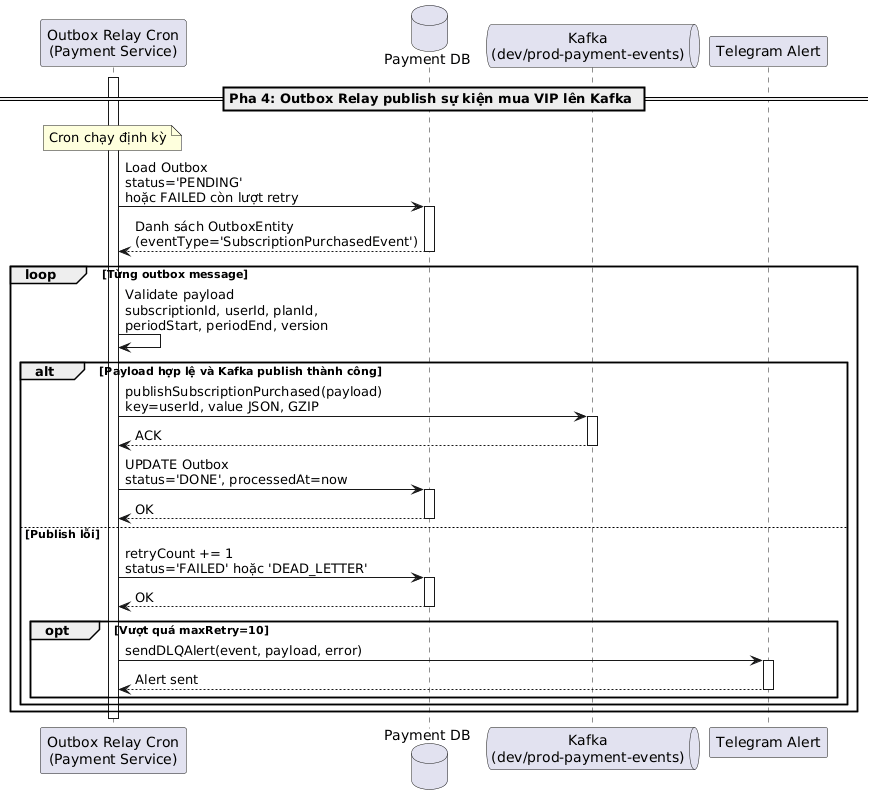
\includegraphics[width=0.85\textwidth]{contents/Sequence/UML-Sequence-PaymentOutboxRelayKafka.png}
\caption{Sơ đồ tuần tự luồng Outbox Relay xuất bản sự kiện VIP}
\end{figure}

\begin{table}[H]
\centering
\renewcommand{\arraystretch}{1.3}

\begin{tabular}{|l|l|p{5cm}|}
\hline
\textbf{Thành phần} & \textbf{Phân loại} & \textbf{Vai trò trong hệ thống} \\ \hline
Outbox Relay Cron & Component & Cron job trong dịch vụ thanh toán, đọc Outbox và điều phối xuất bản sự kiện. \\ \hline
Payment DB & Database & Lưu các trạng thái trong bảng Outbox. \\ \hline
Kafka & Message Broker & Nhận sự kiện thanh toán. \\ \hline
Telegram Alert & External Service & Nhận cảnh báo khi Outbox message vượt quá số lần retry tối đa. \\ \hline
\end{tabular}
\caption{Các thành phần tham gia luồng Outbox Relay xuất bản sự kiện VIP}
\end{table}

\subparagraph{Mô tả tổng quan}

\begin{itemize}

\item \textbf{Quét danh sách sự kiện:}
Tiến trình định kỳ quét bảng sự kiện chờ gửi trong CSDL
để lấy danh sách các sự kiện giao dịch
đang chờ xử lý hoặc đã thất bại
nhưng chưa vượt quá số lần thử lại tối đa.

\item \textbf{Kiểm tra dữ liệu:}
Tiến trình kiểm tra thông tin sự kiện
để đảm bảo dữ liệu hợp lệ.

\item \textbf{Gửi thông điệp sự kiện:}
Tiến trình gửi thông điệp sự kiện mua gói thuê bao VIP thành công
vào hệ thống phát sự kiện.

\item \textbf{Cập nhật kết quả:}
Nếu gửi thành công, tiến trình cập nhật sự kiện sang trạng thái đã hoàn thành.
Nếu xảy ra lỗi, hệ thống tăng số lần thử lại
và chuyển trạng thái sự kiện thành thất bại.
Khi vượt quá số lần thử lại tối đa, sự kiện được đưa vào danh sách lỗi và gửi cảnh báo về nhóm hỗ trợ hệ thống.
\end{itemize}
